% =====================================================================
% Snippet: pipeline-stages.tex
% =====================================================================
% USAGE: N-stage horizontal pipeline with zone tinting, arrows between
% stages, and dataset/info badges below. Copy %% COPY-START / END,
% then replace:
%   - stage list: \def\stages{name/color, name/color, ...}
%   - origin_x, origin_y
%   - stage_W, stage_H: dimensions per stage
%   - arrow_style: connecting arrow style (default arrow)
%
% Colors should be from multi-zone-palette.tex (acaBlue, acaPurple etc.)
% =====================================================================

\documentclass[tikz,border=10pt]{standalone}
\usepackage{xcolor,tikz}
\usetikzlibrary{positioning,calc,arrows.meta,bending}

\definecolor{acaBlueLine}{HTML}{3060A8}
\definecolor{acaBlueBg}{HTML}{DCE6F4}
\definecolor{acaPurpleLine}{HTML}{6E3FA0}
\definecolor{acaPurpleBg}{HTML}{EDE3F6}
\definecolor{acaOrangeLine}{HTML}{D06020}
\definecolor{acaOrangeBg}{HTML}{F9E0D0}
\definecolor{acaGreenLine}{HTML}{389050}
\definecolor{acaGreenBg}{HTML}{DBEDDC}
\definecolor{acaTealLine}{HTML}{1F8F8F}
\definecolor{acaTealBg}{HTML}{D3EBEB}
\definecolor{acaGoldLine}{HTML}{B08820}
\definecolor{acaGoldBg}{HTML}{F4E8CC}
\definecolor{acaGreyLine}{HTML}{606060}

\tikzset{
  pipe arrow/.style={
    -{Stealth[length=4pt 1.0, width'=0pt 0.5]},
    line width=1.0pt, color=acaGreyLine,
    shorten >=2pt, shorten <=2pt,
  },
  stage box/.style={
    rectangle, rounded corners=4pt,
    minimum width=2.0cm, minimum height=1.0cm,
    line width=0.8pt, font=\small\bfseries,
    align=center,
  },
}

\begin{document}
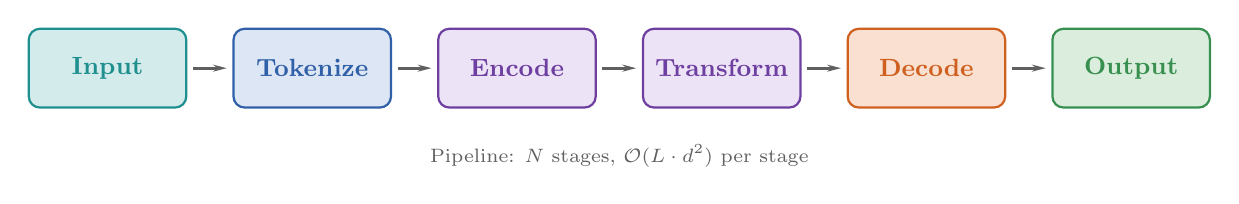
\begin{tikzpicture}

%% COPY-START =========================================================

% --- PARAMETERS ---
% Note: each stage has explicit numeric index (1..N) to avoid
% TeX counter quirks inside foreach. Arrows are drawn pair-by-pair
% via a parallel paired list (must match stage count - 1).
\def\stages{%
  1/Input/acaTealLine/acaTealBg,%
  2/Tokenize/acaBlueLine/acaBlueBg,%
  3/Encode/acaPurpleLine/acaPurpleBg,%
  4/Transform/acaPurpleLine/acaPurpleBg,%
  5/Decode/acaOrangeLine/acaOrangeBg,%
  6/Output/acaGreenLine/acaGreenBg%
}
\def\arrowpairs{1/2, 2/3, 3/4, 4/5, 5/6}  % N-1 pairs for N stages

\def\xO{0}
\def\yO{0}
\def\stageGap{2.6}          % spacing between stage centers

% --- DRAW STAGES ---
\foreach \sidx/\name/\colLine/\colBg in \stages {
  \pgfmathsetmacro\cx{\xO + (\sidx - 1) * \stageGap}
  \node[stage box, fill=\colBg, draw=\colLine, text=\colLine]
    (s\sidx) at (\cx, \yO) {\name};
}

% --- ARROWS BETWEEN STAGES ---
\foreach \a/\b in \arrowpairs {
  \draw[pipe arrow] (s\a.east) -- (s\b.west);
}

% --- INFO BADGE BELOW (optional, customize text) ---
\def\nstages{6}  % hard-coded to match \stages list length above
\pgfmathsetmacro\badgeX{\xO + (\nstages - 1) * \stageGap / 2}
\node[font=\scriptsize, color=acaGreyLine, anchor=north]
  at (\badgeX, \yO - 0.85)
  {Pipeline: $N$ stages, $\mathcal{O}(L \cdot d^2)$ per stage};

%% COPY-END ===========================================================

\end{tikzpicture}
\end{document}
